%!Mode:: "TeX:UTF-8"
\documentclass[a4paper,11pt,UTF8]{ctexart}

\usepackage{indentfirst} %缩进
\usepackage{xeCJK}    %使用系统字体
\usepackage{fancyhdr} %自定义页眉页脚
\pagestyle{empty}                   %不设置页眉页脚
\usepackage{amsmath, amsthm, amssymb, amsfonts} %数学公式
\usepackage[a4paper,left=3cm,right=3cm,top=3cm,bottom=3cm]{geometry}
%\usepackage[tmargin=1in,bmargin=1in,lmargin=1.25in,rmargin=1.25in]{geometry}.
\usepackage{booktabs} %插入表格
\usepackage[section]{placeins} %避免浮动
\usepackage{listings} %插入代码
\usepackage{ctex}     %中文宏包
\usepackage[svgnames, table]{xcolor} %彩色表格
\usepackage{algorithm}          %伪代码
\usepackage{algorithmicx}
\usepackage{algpseudocode}
\usepackage{algorithm,algpseudocode,float}
\usepackage{lipsum}
\usepackage{enumitem}           %调整列举环境
\usepackage{url}
\usepackage{fontspec,xunicode}
\defaultfontfeatures{Mapping=tex-text} %如果没有它,会有一些 tex 特殊字符无法正常使用,比如连字符。

\usepackage{graphicx}
\graphicspath{{imgs/}}

%%%%%%%%%%%%%%%%%%%%%%%%%%%%%%%%%%%%%%%%%%%%%%%%%%%%%%%%%%%%%%%%
% 缩进及行间距
%%%%%%%%%%%%%%%%%%%%%%%%%%%%%%%%%%%%%%%%%%%%%%%%%%%%%%%%%%%%%%%%
\setlength{\parindent}{22pt} %重新定义缩进长度
\setlength{\baselineskip}{20pt}  %定义行间距
%\renewcommand{\baselinestretch}{1.1} %定义行间距

%%%%%%%%%%%%%%%%%%%%%%%%%%%%%%%%%%%%%%%%%%%%%%%%%%%%%%%%%%%%%%%%
% 列表设置
%%%%%%%%%%%%%%%%%%%%%%%%%%%%%%%%%%%%%%%%%%%%%%%%%%%%%%%%%%%%%%%%
\setenumerate{fullwidth,itemindent=\parindent,listparindent=\parindent,itemsep=0ex,partopsep=0pt,parsep=0ex}
\setenumerate[2]{label=\alph*),leftmargin=1.5em}  %二级item设置
\setitemize{itemindent=38pt,leftmargin=0pt,itemsep=-0.4ex,listparindent=26pt,partopsep=0pt,parsep=0.5ex,topsep=-0.25ex}
\setdescription{itemindent=38pt,leftmargin=0pt,itemsep=-0.4ex,listparindent=26pt,partopsep=0pt,parsep=0.5ex,topsep=-0.25ex}

%%%%%%%%%%%%%%%%%%%%%%%%%%%%%%%%%%%%%%%%%%%%%%%%%%%%%%%%%%%%%%%%
% 图的标题行间距设置
%%%%%%%%%%%%%%%%%%%%%%%%%%%%%%%%%%%%%%%%%%%%%%%%%%%%%%%%%%%%%%%%
\newcommand{\bottomcaption}{%
\setlength{\abovecaptionskip}{6pt}%
\setlength{\belowcaptionskip}{6pt}%
\caption}


%%%%%%%%%%%%%%%%%%%%%%%%%%%%%%%%%%%%%%%%%%%%%%%%%%%%%%%%%%%%%%%%
% 字体定义
%%%%%%%%%%%%%%%%%%%%%%%%%%%%%%%%%%%%%%%%%%%%%%%%%%%%%%%%%%%%%%%%
\setmainfont{Times New Roman}  %默认英文字体.serif是有衬线字体sans serif无衬线字体
\setmonofont{Consolas}
\setCJKmainfont[ItalicFont={楷体}, BoldFont={黑体}]{宋体}%衬线字体 缺省中文字体为
\setCJKsansfont{黑体}
\punctstyle{hangmobanjiao}
%-----------------------xeCJK下设置中文字体------------------------------%
\setCJKfamilyfont{song}{SimSun}                             %宋体 song
\newcommand{\song}{\CJKfamily{song}}
\setCJKfamilyfont{fs}{FangSong}                      %仿宋  fs
\newcommand{\fs}{\CJKfamily{fs}}
\setCJKfamilyfont{ktgb}{KaiTi}                      %楷体2312 ktgb
\newcommand{\ktgb}{\CJKfamily{ktgb}}
\setCJKfamilyfont{yh}{Microsoft YaHei}                    %微软雅黑 yh
\newcommand{\yh}{\CJKfamily{yh}}
\setCJKfamilyfont{hei}{SimHei}                              %黑体  hei
\newcommand{\hei}{\CJKfamily{hei}}
\setCJKfamilyfont{hwxk}{STXingkai}                                %华文行楷  hwxk
\newcommand{\hwxk}{\CJKfamily{hwxk}}
%------------------------------设置字体大小------------------------%
\newcommand{\shiyanbaogao}{\fontsize{36pt}{\baselineskip}\selectfont}
\newcommand{\chuhao}{\fontsize{42pt}{\baselineskip}\selectfont}     %初号
\newcommand{\xiaochuhao}{\fontsize{36pt}{\baselineskip}\selectfont} %小初号
\newcommand{\yihao}{\fontsize{28pt}{\baselineskip}\selectfont}      %一号
\newcommand{\erhao}{\fontsize{21pt}{\baselineskip}\selectfont}      %二号
\newcommand{\xiaoerhao}{\fontsize{18pt}{\baselineskip}\selectfont}  %小二号
\newcommand{\sanhao}{\fontsize{15.75pt}{\baselineskip}\selectfont}  %三号
\newcommand{\sihao}{\fontsize{14pt}{\baselineskip}\selectfont}       %四号
\newcommand{\xiaosihao}{\fontsize{12pt}{\baselineskip}\selectfont}  %小四号
\newcommand{\wuhao}{\fontsize{10.5pt}{\baselineskip}\selectfont}    %五号
\newcommand{\xiaowuhao}{\fontsize{9pt}{\baselineskip}\selectfont}   %小五号
\newcommand{\liuhao}{\fontsize{7.875pt}{\baselineskip}\selectfont}  %六号
\newcommand{\qihao}{\fontsize{5.25pt}{\baselineskip}\selectfont}    %七号

%%%%%%%%%%%%%%%%%%%%%%%%%%%%%%%%%%%%%%%%%%%%%%%%%%%%%%%%%%%%%%%%
% 图题字体大小相同
%%%%%%%%%%%%%%%%%%%%%%%%%%%%%%%%%%%%%%%%%%%%%%%%%%%%%%%%%%%%%%%%
\usepackage{caption}
\captionsetup{font={footnotesize}}   % footnotesize = 9pt
\captionsetup[lstlisting]{font={footnotesize}}

%%%%%%%%%%%%%%%%%%%%%%%%%%%%%%%%%%%%%%%%%%%%%%%%%%%%%%%%%%%%%%%%
% 重定义枚举编号为 1),2)...
%%%%%%%%%%%%%%%%%%%%%%%%%%%%%%%%%%%%%%%%%%%%%%%%%%%%%%%%%%%%%%%%
\renewcommand{\labelenumi}{\theenumi)}

%%%%%%%%%%%%%%%%%%%%%%%%%%%%%%%%%%%%%%%%%%%%%%%%%%%%%%%%%%%%%%%%
% 标题名称中文化
%%%%%%%%%%%%%%%%%%%%%%%%%%%%%%%%%%%%%%%%%%%%%%%%%%%%%%%%%%%%%%%%
\renewcommand\figurename{\hei 图}
\renewcommand\tablename{\hei 表}
\renewcommand\lstlistingname{\hei 代码}
\renewcommand{\algorithmicrequire}{\textbf{输入:}}
\renewcommand{\algorithmicensure}{\textbf{输出:}}
\newtheorem{define}{定义}

%%%%%%%%%%%%%%%%%%%%%%%%%%%%%%%%%%%%%%%%%%%%%%%%%%%%%%%%%%%%%%%%
% 代码设置
%%%%%%%%%%%%%%%%%%%%%%%%%%%%%%%%%%%%%%%%%%%%%%%%%%%%%%%%%%%%%%%%
\lstset{
 columns=fixed,
 numbers=left,                                        % 在左侧显示行号
 numberstyle=\tiny\color{gray},                       % 设定行号格式
 frame=single,                                        % 单线背景边框
 breaklines=true,                                     % 设定LaTeX对过长的代码行进行自动换行
 keywordstyle=\color[RGB]{40,40,255},                 % 设定关键字颜色
 numberstyle=\footnotesize\color{darkgray},
 commentstyle=\it\color[RGB]{0,96,96},                % 设置代码注释的格式
 stringstyle=\rmfamily\slshape\color[RGB]{128,0,0},   % 设置字符串格式
 showstringspaces=false,                              % 不显示字符串中的空格
 language=java,                                        % 设置语言
 basicstyle=\linespread{1.0}\xiaowuhao\ttfamily,                      % 字体字号
 %lineskip=10pt,
 %baselinestretch=1,
}

%%%%%%%%%%%%%%%%%%%%%%%%%%%%%%%%%%%%%%%%%%%%%%%%%%%%%%%%%%%%%%%%
% 伪代码分页
%%%%%%%%%%%%%%%%%%%%%%%%%%%%%%%%%%%%%%%%%%%%%%%%%%%%%%%%%%%%%%%%
\makeatletter
\renewcommand{\ALG@name}{算法}
\newenvironment{breakablealgorithm}
  {% \begin{breakablealgorithm}
   \begin{center}
     \refstepcounter{algorithm}% New algorithm
     \hrule height.8pt depth0pt \kern2pt% \@fs@pre for \@fs@ruled
     \renewcommand{\caption}[2][\relax]{% Make a new \caption
       {\raggedright\textbf{\ALG@name~\thealgorithm} ##2\par}%
       \ifx\relax##1\relax % #1 is \relax
         \addcontentsline{loa}{algorithm}{\protect\numberline{\thealgorithm}##2}%
       \else % #1 is not \relax
         \addcontentsline{loa}{algorithm}{\protect\numberline{\thealgorithm}##1}%
       \fi
       \kern2pt\hrule\kern2pt
     }
  }{% \end{breakablealgorithm}
     \kern2pt\hrule\relax% \@fs@post for \@fs@ruled
   \end{center}
  }
\makeatother

% =============================================
% Part 1 Edit the info
% =============================================

\newcommand{\major}{物理学院}
\newcommand{\name}{黄阅迅,李秋阳}
\newcommand{\stuid}{PB18020631,PB18020567}
\newcommand{\group}{20}
\newcommand{\newdate}{\today}


\newcommand{\course}{电子线路实验(1)}
\newcommand{\newtitle}{差动放大器}

%
\newcommand{\p}{\par}
\newcommand{\np}{\par\noindent}

% =============================================
% Part 1 Main document
% =============================================
\begin{document}
\thispagestyle{empty}
\begin{figure}[h]
  \begin{minipage}{0.6\linewidth}
    \centerline{
\includegraphics[width=\linewidth]{logo.png}}
  \end{minipage}
  \hfill
  \begin{minipage}{.4\linewidth}
    \raggedleft
    \begin{tabular*}{.8\linewidth}{ll}
      学院: & \underline\major   \\
      姓名: & \underline\name    \\
      学号: & \underline\stuid   \\
      组号:  & \underline\group   \\
      日期: & \underline\newdate \\
    \end{tabular*}
  \end{minipage}
\end{figure}

\begin{table}[!htbp]
  \centering
  \begin{tabular*}{\linewidth}{llllll}
    课程名称:  \underline\course   \qquad\qquad 实验题目:  \underline\newtitle  
  \end{tabular*}
\end{table}

% =============================================
% Part 2 Main document
% =============================================

\section{实验目的}

请参看预习报告。

\section{实验原理}

请参看预习报告。

\section{实验内容与步骤}
\subsection{实验内容一}
  测量典型差动放大器的参数,并计算共模抑制比。
\subsection{实验步骤一}
\begin{figure}[htbp]
  \centering
  \fbox{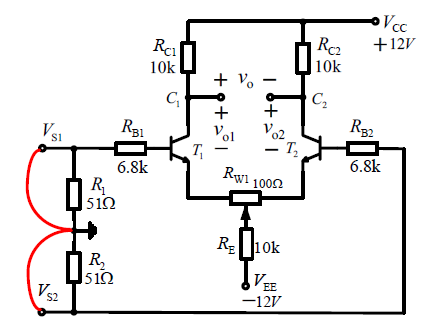
\includegraphics[width=0.5\linewidth]{nStatic.png}}
  \caption{典型差动放大器静态工作点测量示意图}
  \label{fig:nStatic}
  \end{figure}
\begin{enumerate}
  \item 按照图 \ref{fig:nStatic}连接线路,将输入信号接地,调节$R_{w1}$电位器使得$V_{C1}=V_{C2}$。用万用表直流电压
  挡位分别测量差动放大器的静态工作点参数。
  \item 将放大器输入端$V_{s2}$接地,从$V_{s1}$输入正弦信号,调节有效值为$V_{id}=20mVrms$,频率$f=1kHz$。测量差模信号的单端及双端输出信号的有效值并用示波器观察波形。
  \item 将输入端$V_{s1}$和$V_{s2}$两点连接在一起,电阻$R_1$与$R_2$从电路中断开,从$V_{s1}$和$V_{s2}$两端输入$V_{ic}=90mVrms$,频率$f=1kHz$的正弦信号。测量共模信号的单端及双端输出信号的有效值并用示波器观察波形。
  \item 根据测量数据计算单端和双端输出的共模抑制比。
\end{enumerate}
\subsection{实验内容二}
  将电阻$R_E$改为镜像恒流源,测量构成差动放大器的参数,并计算共模抑制比。
\subsection{实验步骤二}
\begin{figure}[htbp]
  \centering
  \fbox{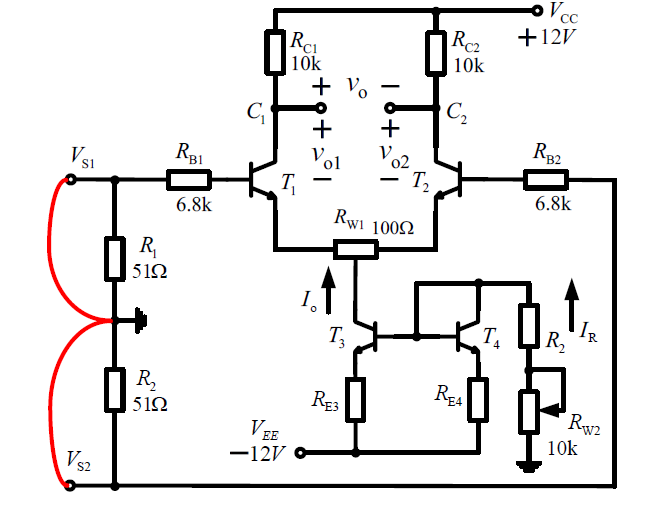
\includegraphics[width=0.5\linewidth]{sStatic.png}}
  \caption{恒流源差动放大器静态工作点测量示意图}
  \label{fig:sStatic}
  \end{figure}
\begin{enumerate}
  \item 按照图 \ref{fig:sStatic}连接线路,将输入信号接地,调节恒流源$R_{w2}=10k$电位器使得$I_0=1mA$即$V_{RC1}=5V$。用万用表直流电压
  挡位分别测量差动放大器的静态工作点参数。
  \item 将放大器输入端$V_{s2}$接地,从$V_{s1}$输入正弦信号,调节有效值为$V_{id}=20mVrms$,频率$f=1kHz$。测量差模信号的单端及双端输出信号的有效值并用示波器观察波形。
  \item 将输入端$V_{s1}$和$V_{s2}$两点连接在一起,电阻$R_1$与$R_2$从电路中断开,从$V_{s1}$和$V_{s2}$两端输入$V_{ic}=90mVrms$,频率$f=1kHz$的正弦信号。测量共模信号的单端及双端输出信号的有效值。
  \item 根据测量数据计算单端和双端输出的共模抑制比。
\end{enumerate}

\section{实验数据处理与分析}
\subsection{实验内容1.1}
  实验测得的静态工作点数据如表 \ref{tab:nSTab}所示。可见得到的数据都对称点的值都较为接近,比较理想。
  \begin{table}[!h!tbp]
    \caption{典型差动放大器静态工作点数据}\label{tab:nSTab}
      \centering
      \begin{tabular}{|l|c|c|c|c|c|c|}
      \hline
      数据 &$V_{C_1}$&$V_{C_2}$&$V_{E_1}$&$V_{E_2}$&$V_{B_1}$&$V_{B_2}$         \\ \hline
      值   &$6.185V$&$6.187V$&$-0.638V$&$-0.643V$&$-13.76mV$&$-15.40mV$     \\ \hline
    \end{tabular}
    \end{table}
\subsection{误差分析1.1}
  上述静态工作点数据,理论上对称点应完全一致,但由于实验误差,无法做到。但保证了相差小于$20mV$,从原理上可以接受,下面理论计算
  静态工作点数值。计算中采用值为$\beta=150,r_{bb'}=300\Omega,U_{BE}=0.7V$
  \begin{equation}
    \begin{aligned}
      I_{B}&=\frac{-U_{EE}-U_{BE}}{R_{B_1}+2(1+\beta)R_E+(1+\beta)\frac{R_{W_1}}{2}}=3.74\times10^{-3}mA\\
      I_{C}&=\beta I_{B}=0.561mA\\
      U_{CE}&=U_{CC}+U_{EE}-I_CR_C-2I_CR_E-I_C\frac{R_{W_1}}{2}=7.14V\\
      U_C&=U_CC-I_CR_C=6.39V\\
      U_E&=U_C-U_{CE}=-0.75V\\
      U_B&=U_E+U_{BE}=-0.05V\\
      r_{be}&=r_{bb'}+\frac{26mV}{I_B(mA)}=7.25k\Omega
    \end{aligned}
  \end{equation}
  由此可以计算出分别的相对误差(对称点取平均值)为:
  \begin{equation}
    \begin{aligned}
      \left |\frac{\Delta U_C}{U_C}\right |&=3.2\%\\
      \left |\frac{\Delta U_E}{U_E}\right |&=14\%\\
      \left |\frac{\Delta U_B}{U_B}\right |&=71\%
    \end{aligned}
  \end{equation}

  可见,除$U_C$值外,其他静态工作点值基本上只有数量级正确。这主要是因为另外两个点值基本上在$1mV$范围,因此
毫伏表的测量相当不精确造成的。但$U_C$的误差较小,说明了实验与理论基本上还是对应的。同时理论中采用了大量的近似,并且所选取
的参数值可能也与实际由偏差,因此这样的误差可以接受。实际上,对称点的电压值难以调整至一致也说明了实验的电压误差基本上是在$20mV$这个数量级的。
\subsection{实验内容1.2}
实验中测量得到的数据如表 \ref{tab:ndTab}所示。可见在此精度范围下,单端差模输出的有效值的绝对值基本一致。其波形图如附图1所示。可见两端的差模输出信号的反向的。
\begin{table}[!h!tbp]
  \caption{典型差动放大器差模输出数据}\label{tab:ndTab}
    \centering
    \begin{tabular}{|l|c|c|c|c|}
    \hline
    数据 &$V_{S_1}$&$V_{od_1}$&$V_{od_2}$&$V_{od}$         \\ \hline
    值   &$19.92mV$&$-808mV$&$+808mV$&$-1.610V$     \\ \hline
  \end{tabular}
  \end{table}
由此可以计算出差模信号增益为:
\begin{equation}
  \begin{aligned}
    \left |A_{ods}\right |=40.6\\
    \left |A_{od}\right |=80.8
  \end{aligned}
\end{equation}
\subsection{误差分析1.2}
可见实际上$v_{od}$的测量值并不完全等于$v_{od1}-V_{od2}$,但实际上这就是毫伏表读数误差造成的。
为计算理论值,画出单边小信号等效电路如图 \ref{fig:ndSmallSignal}所示。($R_b$与$R_w$未画出,认为负载$R_L\rightarrow\infty$)
\begin{figure}[htbp]
  \centering
  \fbox{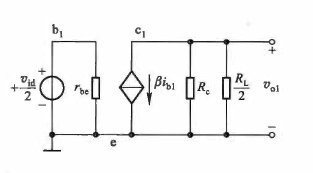
\includegraphics[width=0.5\linewidth]{ndSmallSignal.png}}
  \caption{典型差动放大器差模输出单边小信号模型}
  \label{fig:ndSmallSignal}
  \end{figure}
则可以求出输出参数为:
\begin{equation}
  \begin{aligned}
    \left | A_{vd}\right |&=\frac{\beta R_C\parallel\frac{R_L}{2}}{R_{B_1}+r_{be}+(1+\beta)\frac{R_{W_1}}{2}}=70.0\\
    \left | A_{vds}\right |&=\left |\frac{A_{vd}}{2}\right |=35.0
  \end{aligned}
\end{equation}
则可求出相对误差为:
\begin{equation}
  \begin{aligned}
    \left |\frac{\Delta A_{vd}}{A_{vd}}\right |&=15\%\\
      \left |\frac{\Delta A_{vds}}{A_{vds}}\right |&=16\%\\
  \end{aligned}
\end{equation}
首先,可见差模双端输出放大倍数并不是严格的单端输出的两倍。同时测量值与理论值偏差较大,推测是使用计算的$\beta$与$r_{bb'}$不准所导致的。
这在静态工作点时已有体现,这个误差经过放大变得更加大。同时使用的元件也有一定的误差,小信号分析本身也具有一定误差,并未考虑频率响应。
\subsection{实验内容1.3}
实验测得的共模输出数据如表 \ref{tab:ncTab}所示。而输出波形如附图2所示。可见共模输出电压较小。

\begin{table}[!h!tbp]
  \caption{典型差动放大器共模输出数据}\label{tab:ncTab}
    \centering
    \begin{tabular}{|l|c|c|c|c|}
    \hline
    数据 &$U_{i}$&$U_{oc_1}$&$U_{oc_2}$&$U_{oc}$         \\ \hline
    值   &$90.1mV$&$-43.9mV$&$-46.8mV$&$1.610mV$     \\ \hline
  \end{tabular}
  \end{table}
则可以计算出共模电压增益为(单端输出时取平均值):
\begin{equation}
  \begin{aligned}
    \left | A_{ucs}\right |&=0.503\\
    \left | A_{uc}\right |&=0.0306
  \end{aligned}
\end{equation}
结合上一实验内容,可以算出差模抑制比为:
\begin{equation}
  \begin{aligned}
    K_{CMRs}&=80.7\\
    K_{CMR}&=2.64\times10^{3}
  \end{aligned}
\end{equation}
\subsection{误差分析1.3}
同样有,单端输出和双端输出电压值并不完全匹配的问题。
单端输出时半边小信号模型如图\ref{fig:ncSmallSignal}所示。($R_b$与$R_w$未画出,认为负载$R_L\rightarrow\infty$)
\begin{figure}[htbp]
  \centering
  \fbox{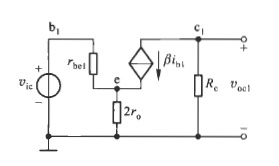
\includegraphics[width=0.5\linewidth]{ncSmallSignal.png}}
  \caption{典型差动放大器共模输出单边小信号模型}
  \label{fig:ncSmallSignal}
  \end{figure}
则可以求出共模输出参数以及结合上一内容模型可以算出差模抑制比为
\begin{equation}
  \begin{aligned}
    \left | A_{vcs}\right |&\approx\frac{R_c\parallel R_L}{2R_E}=0.500\\
    \left | A_{vc}\right |&=0.00\\
    K_{CMRs}&=\left |\frac{A_{vds}}{A_{vcs}}\right |=70.0\\
    K_{CMR}&=\infty
  \end{aligned}
\end{equation}
可见,双端输出时的抑制比并不可能做到理想的正无穷程度,共模输出增益也不可能是0,但前者也非常大,后者也相当小,比较符合理论预测。
其他量的相对误差为:
\begin{equation}
  \begin{aligned}
      \left |\frac{\Delta A_{cds}}{A_{cds}}\right |&=0.6\%\\
      \left |\frac{\Delta K_{CMRs}}{K_{CMRs}}\right |&=15\%
  \end{aligned}
\end{equation}
可见,共模单端输出的相对误差意外得小,这是因为其计算时几乎没有用到三极管的预设参数。侧面证明,计算误差来源可能主要是三极管的参数不准。
单端共模抑制比的误差仍较大,原因如前所述。

\subsection{实验内容2.1}
实验测得的静态工作点数据如表 \ref{tab:sSTab}所示。可见得到的数据都对称点的值都较为接近,比较理想。
  \begin{table}[!h!tbp]
    \caption{恒流源差动放大器静态工作点数据}\label{tab:sSTab}
      \centering
      \begin{tabular}{|l|c|c|c|c|c|c|c|}
      \hline
      数据 &$V_{C_1}$&$V_{C_2}$&$V_{E_1}$&$V_{E_2}$&$V_{B_1}$&$V_{B_2}$&$R_{W2}$         \\ \hline
      值   &$6.915V$&$6.909V$&$-0.630V$&$-0.635V$&$-11.98mV$&$-13.45mV$&$4.14k\Omega$     \\ \hline
    \end{tabular}
    \end{table}
可见,数值上的对称性仍有缺陷。
\subsection{误差分析2.1}
下面理论计算静态工作点值,有:
\begin{equation}
  \begin{aligned}
    I_C=I_0/2=0.500 mA\\
    U_C=U_CC-I_CR_C=7.00V\\
    r_{be}=r_{bb'}+\beta\frac{26mV}{I_C}=8.10k\Omega\\
    U_{B}=-I_bR_B=-0.0227V\\
    U_{E}=U_{B}-U_{BE}=-0.723V
  \end{aligned}
\end{equation}
则可以分别计算出相对误差:
\begin{equation}
  \begin{aligned}
    \left |\frac{\Delta U_C}{U_C}\right |&=1.2\%\\
    \left |\frac{\Delta U_E}{U_E}\right |&=13\%\\
    \left |\frac{\Delta U_B}{U_B}\right |&=44\%
  \end{aligned}
\end{equation}
相对典型差分放大器而言,相对误差有所下降,因为此时理论计算的依赖主要跟$I_0$有关,而其为实验调制出来的,从这里可以猜测误差来源于参数$U_{BE}$的贡献可能最大。
基本上精度还能接受,$U_C$误差比较小。
\subsection{实验内容2.2}
实验中测量得到的数据如表 \ref{tab:sdTab}所示。可见在此精度范围下,单端差模输出的有效值的绝对值基本一致。其波形图如附图1所示。可见两端的差模输出信号的反向的。
\begin{table}[!h!tbp]
  \caption{恒流源差动放大器差模输出数据}\label{tab:sdTab}
    \centering
    \begin{tabular}{|l|c|c|c|c|}
    \hline
    数据 &$V_{S_1}$&$V_{od_1}$&$V_{od_2}$&$V_{od}$         \\ \hline
    值   &$19.85mV$&$-760mV$&$+767mV$&$-1.52V$     \\ \hline
  \end{tabular}
  \end{table}
  可见对称度较典型的低,但$V_{od}$的值与单端输出的值匹配较好。
  \begin{equation}
    \begin{aligned}
      \left |A_{ods}\right |=38.5\\
      \left |A_{od}\right |=76.9
    \end{aligned}
  \end{equation}
\subsection{误差分析2.2}
理论分析与分析1.2相似,小信号模型也类似,故不加赘述。
\begin{equation}
  \begin{aligned}
    \left | A_{vd}\right |&=\frac{\beta R_C\parallel\frac{R_L}{2}}{R_{B_1}+r_{be}+(1+\beta)\frac{R_{W_1}}{2}}=66.8\\
    \left | A_{vds}\right |&=\left |\frac{A_{vd}}{2}\right |=33.4
  \end{aligned}
\end{equation}
则可求出相对误差为:
\begin{equation}
  \begin{aligned}
    \left |\frac{\Delta A_{vd}}{A_{vd}}\right |&=13\%\\
      \left |\frac{\Delta A_{vds}}{A_{vds}}\right |&=13\%\\
  \end{aligned}
\end{equation}
问题与典型时一致,基本上实验测得的偏大,显然应该与三极管参数相关。
\subsection{实验内容2.3}
实验测得的共模输出数据如表 \ref{tab:ncTab}所示。而输出波形由于输出已十分微弱,示波器显示已没有测量意义。

\begin{table}[!h!tbp]
  \caption{典型差动放大器共模输出数据}\label{tab:ncTab}
    \centering
    \begin{tabular}{|l|c|c|c|c|}
    \hline
    数据 &$U_{i}$&$U_{oc_1}$&$U_{oc_2}$&$U_{oc}$         \\ \hline
    值   &$89.9mV$&$-1.000mV$&$-1.036mV$&$0.00mV$(测量精度下)     \\ \hline
  \end{tabular}
  \end{table}
则可以计算出共模电压增益为(单端输出时取平均值):
\begin{equation}
  \begin{aligned}
    \left | A_{ucs}\right |&=0.0111\\
    \left | A_{uc}\right |&=0.00
  \end{aligned}
\end{equation}
结合上一实验内容,可以算出差模抑制比为:
\begin{equation}
  \begin{aligned}
    K_{CMRs}&=3.47\times10^3\\
    K_{CMR}&=\infty
  \end{aligned}
\end{equation}
\subsection{误差分析2.3}
为计算共模输出,需要先求出恒流源等效电阻。但由于三极管参数未知,取$r_{ce}=100k\Omega$,则有
\begin{equation}
  \begin{aligned}
    R_B&\approx(R+R_{W2})\parallel R_{E4}=1.64k\Omega\\
    r_{be3}&=r_{bb'}+(1+\beta)\frac{26mV}{I_{E3}mA}=4.23k\Omega\\
    R_e'&=r_{ce}(1+\frac{\beta R_{E_3}}{r_{be3}+R_{E3}+R_{B}})=3.91M\Omega
  \end{aligned}
\end{equation}
则由此计算出的共模增益以及抑制比为
\begin{equation}
  \begin{aligned}
    \left | A_{vcs}\right |&\approx\frac{R_c\parallel R_L}{2R_e'}\approx1\times10^{-3}\\
    \left | A_{vc}\right |&=0.00\\
    K_{CMRs}&=\left |\frac{A_{vds}}{A_{vcs}}\right |=3.34\times10^{4}\\
    K_{CMR}&=\infty
  \end{aligned}
\end{equation}
可见,基本上单端输出时数量级上差了一个数量级,故不再计算相对误差。这是因为此时的测量mV级已经相当不准确了,并且理论计算时要考虑多一个三极管,其所取
参数基本上也不确定,由此造成的估计误差是相当大的。从测量数据上看,实际的$r_{ce}$可能并没有到几百千欧,由此造成的误差应该非常非常大。但在当前精度下,其双端输出抑制比已经趋向
正无穷,可以认为还是符合要求的。
\section{实验总结}
本次实验测量了差动放大器的典型形态和电流源形态。可见使用恒流源作为负载之后,共模抑制比大幅度上升,这是因为恒流源等效输出电阻是非常大的。从理论分析上讲,
与实验相比,精度比较一般。但在当前实验条件以及测量精度下,可以认为还是符合条件的,因此基本上的结果还是符合预期。
\section{实验思考题}
\subsection{为什么要对差分放大器进行调零,在实验中是否非常重要?}
\np \textbf{答:}
\p 理论上电路的左右两端需要保持完全一致,才能保证在零输入时输出为 0,但实际上,因为左右元件的参数不能做到完全一致,所以 需要加入一个可调的元件来修正这种误差。
\p 如果未进行调零或者调零调的不精确,那么在输入共模信号时,元件不对称带来的误差会使得 $u_{c1}$ 与 $u_{c2}$ 误差变大。这会使得 $u_c$ 变大。因为共模输出电压本来应该很小(1mV量级),如果这个值变大了,那么 $K_{CMR}=\frac{|u_d|}{|u_c|}$ 会变大非常多。这也意味着差动放大器的共模抑制比急剧下降。本来差分放大器就是用来抑制共模影响信号的(如零漂、温漂),这些误差值本来也不是太大。假如因为差动放大器未调零而使得输出共模信号很大,那么使用差动放大电路就没有任何优势了。

\subsection{差分放大器的差模输入电压是与输入电压的差还是与输入电压成正比?}
\np \textbf{答:}
\p 假设输出是双端的,但值不相同,为 $u_{i1}$ 和 $u_{i2}$(单端输入是包括在内的,只需要令其中一个电压为 0)。
\p 那么共模信号为 $u_c=\frac{u_{i1}+u_{i2}}{2}$,差模信号为 $u_d=\frac{u_{i1}-u_{i2}}{2}$,输入信号是二者叠加。而输出信号中共模成分基本被抑制,仅剩下差模成分,假设单端输出差模放大系数为 $A_{ds}$,那么输出电压为 $u_o=A_{ds}\cdot 2u_d=A_{ds}(u_{i1}-u_{i2})$。所以显然输出电压是与输入电压的差值成正比的。只放大差模信号,这也正是使用差动放大器的优势所在。


\subsection{典型差动放大电路与恒流源差动放大电路在观测 $u_{c1}$ 与 $u_{c2}$ 的波形时,其大小、极性及共模抑制比 $K_{CMR}$ 有何区别?为什么?}
\np 答:
\p 在共模时,只需要考虑一半的电路,恒流源等效于一个大电阻 $R$。如图所示:
\begin{figure}[H]
 \centering
 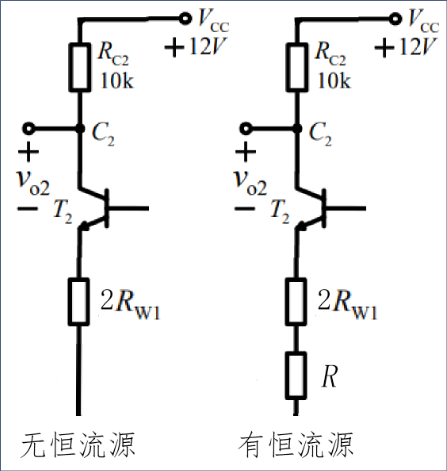
\includegraphics[width=3.5cm]{CCircuit}
 \caption{左边无恒流源,右边有恒流源}
 \label{fig:add-3}
\end{figure}
\p 其交流小信号模型为:
\begin{figure}[H]
 \centering
 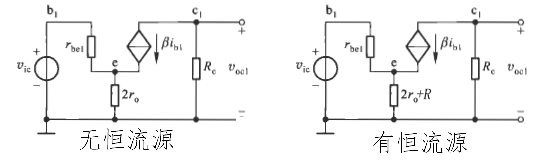
\includegraphics[width=10cm]{CCircuitSmallSignal}
 \caption{左边无恒流源,右边有恒流源}
 \label{fig:add-3-ss}
\end{figure}
\p 容易计算出放大系数:
\begin{itemize}
 \item 无恒流源:
 \np 
 \[ A_{vc}=\frac{-(\beta+1)R_c}{r_{be}+(1+\beta)\cdot 2r_o} \]
 \item 有恒流源:
 \np
 \[ A_{vc}=\frac{-(\beta+1)R_c}{r_{be}+(1+\beta)\cdot(2r_o+R)} \]
\end{itemize}
\p 因为 $R$ 是一很大的电阻,所以有恒流源时 $A_{vc}$ 比无恒流源时小得多,因此起到了进一步抑制共模信号的作用,可以进一步提高 $K_{CMR}$。
\p 综上,根据理论,加入恒流源后,共模输出信号显著减小,极性不变,共模抑制比显著提高。
\p 实际实验时,通过加入恒流源,确实能把 $u_{co}$ 从约 1mV 降到 0(小于毫伏表量程,也无法用示波器看见)。$K_{CMR}$ 急剧提高,直至近乎 $+\infty$。示波器上图像是 0 附近模糊的一片,并没有清晰的图像(参见 \ref{fig:add-3-real}),据估计,可能是因为输出信号太小,噪声等干扰信号占据了主导地位。所以,无法验证两种输出信号是否极性一致。
\begin{figure}[H]
 \centering
 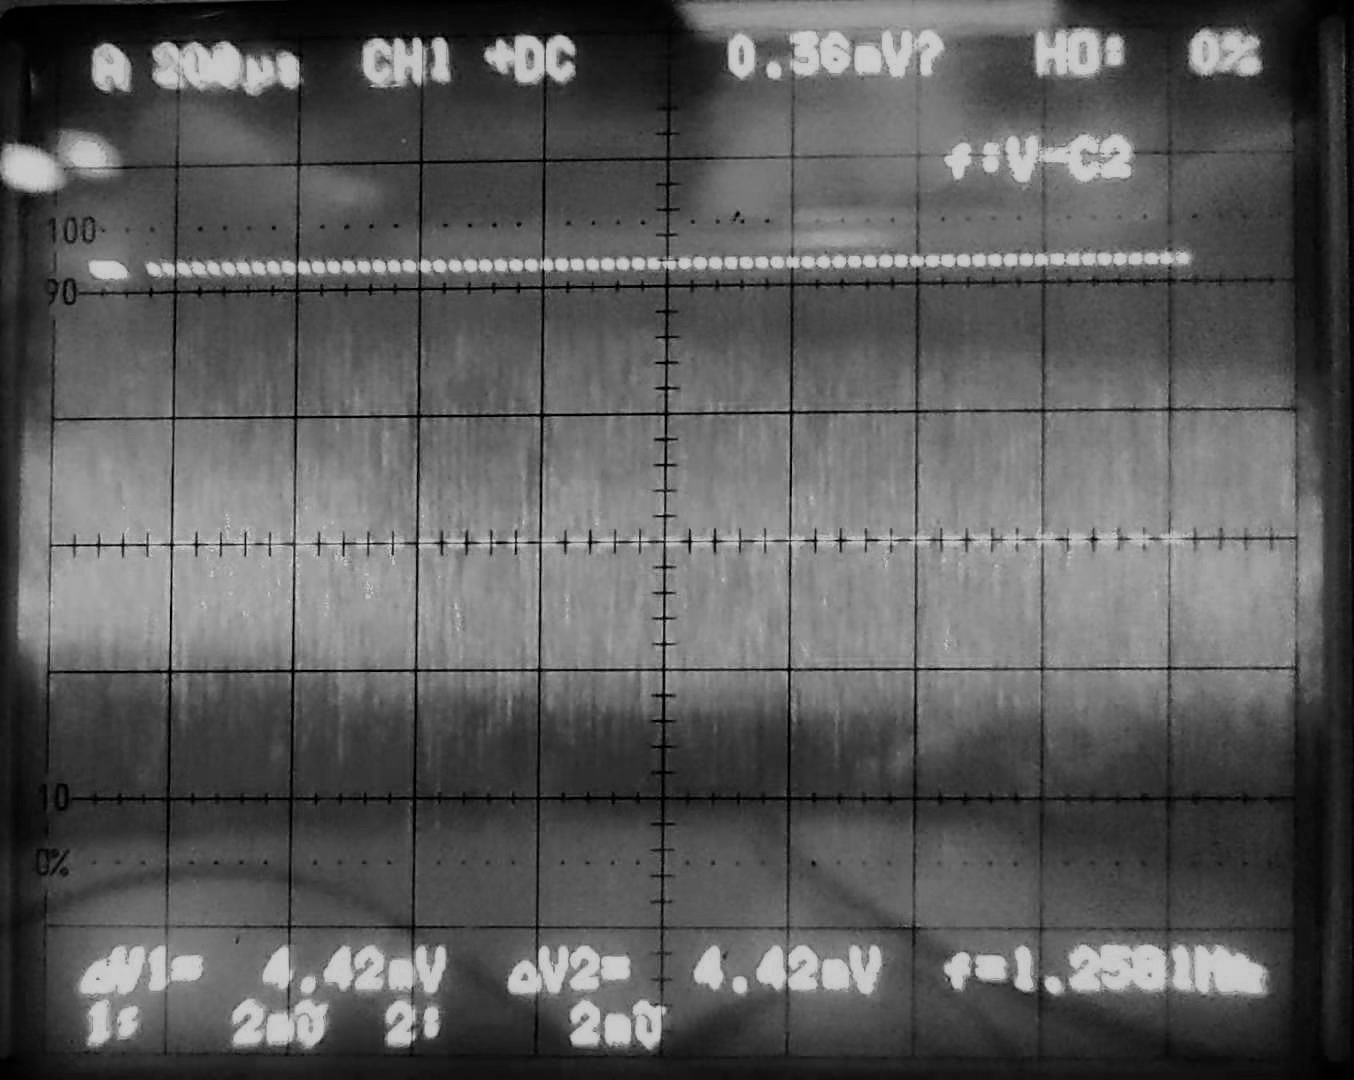
\includegraphics[width=6cm]{RealImage}
 \caption{在有恒流源时,实际示波器上共模输出信号的图像}
 \label{fig:add-3-real}
\end{figure}


\end{document}
